\section{Android  を標的にしたマルウェア}
本研究では,Android を標的にしたマルウェアの中で,悪意ある Android アプリを対象とする.\ref{sec:malware} では,悪意あるアプリの挙動,不正な振る舞いをするためにどのような方法をとっているのかについて説明する.また,マルウェアの例の 1 つとして,GoldDream の挙動を説明する.\ref{sec:andrapp} では,基本的な Android アプリの構成について説明する.Android アプリの概要を示している AndroidManifest.xml とアプリの実行ファイルである,classes.dex について説明する.
\subsection{悪意ある Android  アプリ}
\label{sec:malware}
マルウェアの主な挙動として,個人情報の盗難と不正な金銭請求がある.個人情報に関して言えば,デスクトップ PC やノートパソコンに比べ,スマートフォンは,電話帳,メールなど個人情報のデータの量が多いため,攻撃者の標的になりやすいのは明らかである.スマートフォンでもネットサービス等で銀行口座の操作ができるため,スマートフォンのブラウザに銀行アカウントのパスワードが残っている可能性もある.もし銀行アカウントのパスワードが盗まれた場合,多額の被害を生んでしまうおそれがある.ユーザ自身の情報だけでなく,端末の情報,IMEI(端末識別番号),SIM カードの情報, GPS の位置情報なども盗まれている.金銭を不正に請求するための攻撃方法として,SMS (Short Message Service) を使ったものがある.SMS を使った攻撃の様子を 図\ref{SmsAttack} に示す.SMS Premium Service は,ある番号へ SMS を送ることで音楽や動画などのコンテンツを買うことができるサービスである.この攻撃は Premium Service のように,マルウェアが攻撃者たちの番号へ SMS を送信することで,ユーザーに課金させる方法だ,その課金は携帯電話の料金の支払いと同時に行われ,そこで支払われた料金の一部が攻撃者たちに支払われる.ユーザはその支払い請求が来るまで SMS が送られたことに気づかない.通常の Premium Service ではユーザに支払い確認のメッセージがくるのだが,マルウェアはこれをブロックするためだ.

マルウェアが先に述べたような攻撃をするための方法を 2 つ挙げる.1つは,外部からの遠隔操作だ  \cite{remotectrl} .マルウェアは外部サーバからの命令を受け取り,実行する.あるマルウェアがインストールされると,外部のサーバから暗号化されたスクリプトを受け取り,その復号,実行するという例もある.この手法を使うと,マルウェアを検知するソフトウェアを回避することもできる.なぜなら,公式アプリストア (Google Play)  にアップロードされた時点では不正な動きをするコードをマルウェア自身は何も持っていないため,検知されないからだ.外部から得たスクリプトは DexClassLoader というクラスローダによりアプリケーションに組み込まれていないファイルを読み込むことができる.もう一つは,Android OS の脆弱性をつくことで,特権レベルを上げることである.不正にマルウェア自身の特権レベルを上げるマルウェアの中には root 権限を奪うものもある.マルウェアに root 権限を奪われてしまうと,ユーザが抵抗できる余地は少ないため,悪用されると非常に危険である.マルウェアの 1 つである,AndroidDefender \cite{sopho} は,表向きにはウイルス対策アプリとなっている.AndroidDefender が起動すると,それは感染した端末から電話をかけられなくしたり,さまざまなアプリケーションへのアクセスを制限させる.その後,AndroidDefender は端末を修復するためにユーザに大金を要求する.
 
実際のマルウェアの例として,GoldDream を紹介する.GoldDream は端末情報を流出させるために,電話の発着信などのイベントを監視し,外部へと送信する. そこで,GoldDream の挙動について説明する.GoldDream はSMS の受信,電話の発着信があると,バックグラウンドでユーザに気づかれることなく起動される.GoldDream はレシーバを登録することで,これらの着信が来た時に Android OS が出す通知を受け取れるようにしている.SMS を受信した際は,受信したメッセージの送り元のアドレス,内容,タイムスタンプを収集する.電話の発着信の場合も同様に,電話番号やタイムスタンプといった情報が GoldDream によって集められる.なぜこのような情報をマルウェア作成者が盗もうとするかというと,この情報を用いることで,他の端末へ攻撃を拡大できるためである.例えば,他の端末の情報を得ることができれば,感染した端末から他端末へマルウェアのダウンロードリンクを載せたメッセージなどを送ることができる.これらの情報は一度ローカルファイルに保存された後,外部のサーバへ送信される.GoldDream は外部サーバからコマンドを受け取り,実行する.サーバから受け取るコマンドは,次の 4つである.1)SMS をバックグラウンドで送信する,2)電話を発信する,3)アプリをインストール,アンインストールする,4)ファイルをサーバへアップロードする.ファイルをアップロードするコマンドは端末の情報を送信するために用いられる.

\begin{figure}[t]
\begin{center}
\graphicspath{{./epsfiles/}}
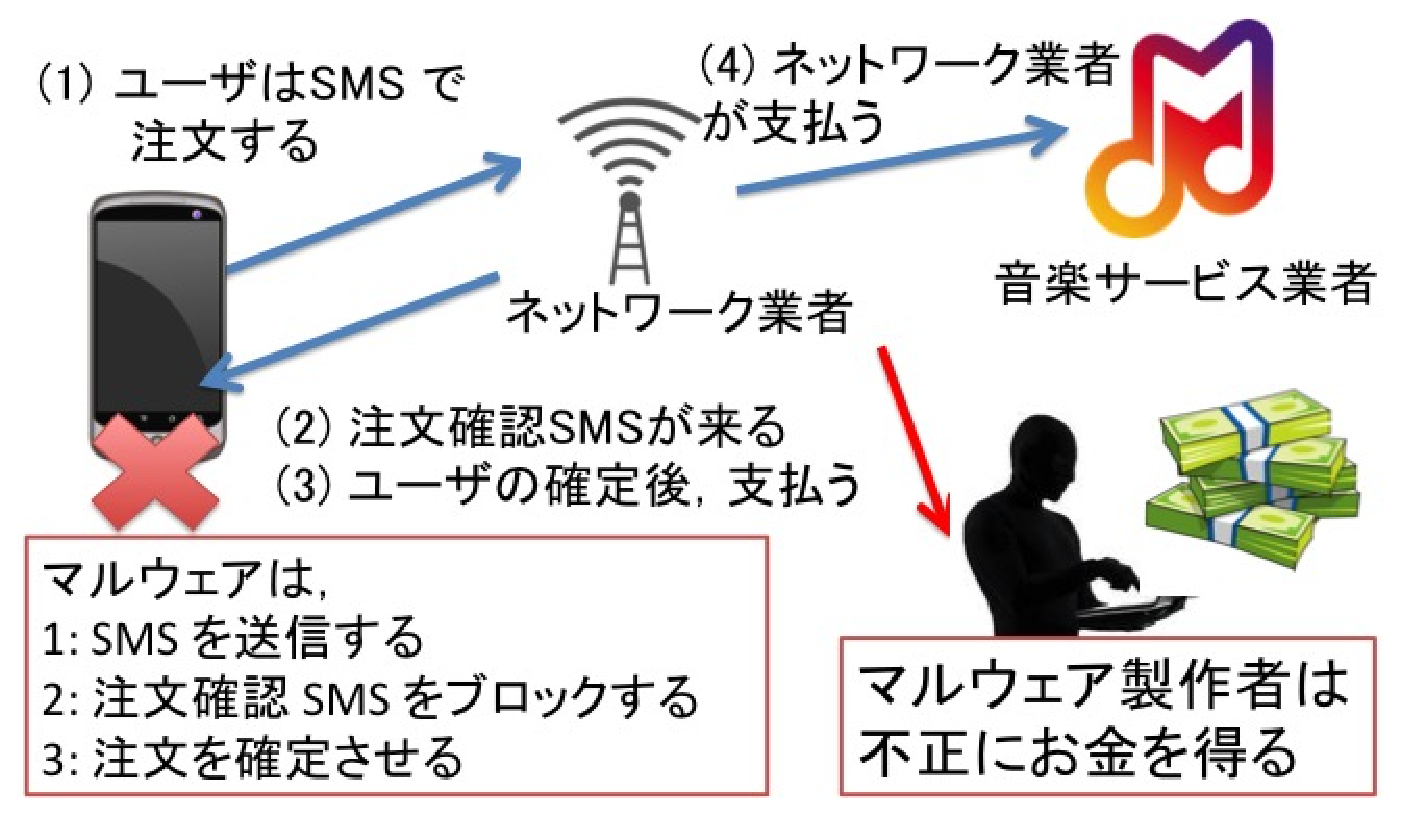
\includegraphics[ scale = 0.4]{sms3.eps}
\end{center}
\caption{SMS を使った攻撃}
\label{SmsAttack}
\end{figure}

\subsection{Android アプリの構成}
\label{sec:andrapp}
1 つの Android アプリは1 つの APK ファイル (.apk) となってまとめられている.Androidのアプリを実行するためには,異なる種類の複数のファイルが必要である.例えば,AndroidManifest.xml, 画像,レイアウトファイル(png, jpg, xml, etc),classes.dex, アプリの証明書,である.これらを1 つのファイルに ZIP 形式でまとめたものが APK ファイルである.そのため,zip ファイルと同様に解凍,圧縮,中身の入れ替えができる.そのため,.zip ファイルを解凍するのと同様, unzip コマンド で APK ファイルを解凍することができる.APK ファイルを解凍すると,AndroidManifest.xml, classes.dex, res ディレクトリ,META-INF ディレクトリが展開される.res ディレクトリには,アプリのアイコン画像,アプリ実行時に画面上に表示する画像ファイルが入っている.META-INF ディレクトリにはアプリの証明書のファイルがある.ただし,unzip コマンドで解凍した場合,AndroidManifest.xml はバイナリのままであるため,このファイルの中身を見たい場合は,apktool \cite{apktool} というツールを使う必要がある.
なぜこれらのファイルを一つの APK ファイルにまとめないといけないかというと,他のアプリも同じファイル名を用いているためだ.どのアプリも必ず AndroidManifest.xml と classes.dex の 2 つのファイルを持っている.そのため,これらのファイルはアプリごとにまとめて端末上にインストールされる必要性がある. そうすることで,Android OS はアプリケーションを管理することができる.

AndroidManifest.xml とはアプリの基本的な情報が書かれている XML 形式のファイルである.あるゲームアプリの AndroidManifst.xml の例を図\ref{manif} に示す.アプリのパッケージ名,アプリが使用する権限,アプリが起動した時に最初に実行されるクラス,などが記されている. パッケージ名は OS がアプリを識別する名前である.図\ref{manif} の 2 行目に.このアプリのパッケージ名 (com.gamelio.DrawSlasher) が書いてある.待ち受け画面で,アイコンの下に表示される名前とは異なる.例えば,Facebook,Instagram の Android アプリの場合はそれぞれ, com.facebook.katana,com.instagram.android となっている.一般的にアプリを使用している分には,ユーザはパッケージ名について気にする必要がないので,使用していてアプリのパッケージ名を目にすることはまずない.ただし,adb (Android Debug Bridge) を用いてターミナルからアプリを手動でアンインストールする場合は,パッケージ名を特定する必要がある.OS monitor という Android のシステム状況を確認できるアプリを使うと,AndroidManifest.xml を見なくても,実行中のアプリのパッケージ名を端末上で見ることができる.Androidのアプリは OS から権限を得ないと実行できないことがいくつもある.電話の着発信,SMS の送受信, インターネットへの接続などである.AndroidManifest.xml に記すことにより,アプリはその権限を得る.これらの機能をアプリで実行するためには,必ず AndroidManifest.xml に宣言しないといけない.図\ref{manif} の中では,24 行目から38 行目にかけてこのアプリの権限が書かれている.さらに,マルウェアの AndroidManifest.xml を得ることができれば,どのようなことをしようとしているのかがわかる.表向きは電話帳のデータとは関係の無いアプリであるのに,AndroidManifest.xml で電話帳へのアクセスの権限を要求していたら,何らかの不正な動きをするアプリである可能性であることが高い. 図\ref{manif} の 34 行目には,電話をかけるための権限である,CALL\_PHONE が宣言されている.このアプリがマルウェアではない,安全なゲームアプリであるとすれば,電話を発信する必要はない.つまり,このアプリは電話をかけることで何らかの不正な動きをする可能性が高い.また,AndroidManifest.xml ではアプリが起動したときに最初に実行する activity を指定する必要がある.図\ref{manif} の 7 行目から,最初に実行される activity は com.Claw.Android.ClawActivity ということがわかる.この指定が無いと Android OS はどこから実行すればよいかわからない.activity とは 1 画面を表すクラスであり,Android アプリ内で画面が変わるということは,他の activity に変わる(遷移する)ということである.画面内でボタンなどを表示させたいときは,android.Activity クラスをオーバーライドして,実装する.このように,AndroidManifest.xml はアプリの大まかな概要を示している.

アプリの画像ファイルが入っている  res (resource) ディレクトリ内には様々なファイルがあり,その種類に応じて配置されるディレクトリが決まっている \cite{resource} . 図\ref{res} は,あるアプリの res ディレクトリの構成を示したものである.layout  ディレクトリでは,ユーザインターフェース (以下 UI) のレイアウトを定義する XML ファイルが入っている.レイアウトリソースファイルはアプリの activity の UI の構成を決めている.例えば,テキストを表示する領域を表す TextView の縦幅と横幅の具体的な値が記されている.drawable ディレクトリには画像ファイル (.png, .jpg, gif etc) と形状などを定義した XML ファイルがある.drawable ディレクトリにある XML ファイルはボタンを押した時などの状態変化のために用いる.図\ref{res} では,drawable ディレクトリがいくつも分かれている.これは,ことなる解像度に対応するためである.ldpi は Low-density,,mdpi は Medium-density,xhdpi は Extra-high-density, xxhdpi は Extra-extra-high-density を表す.menu ディレクトリにはアプリのメニューの内容を定義する XML ファイルが.values  ディレクトリには文字列,数値,色などの値を定義する XML ファイルが入っている.

classes.dex は,Android アプリの DEX コード実行ファイルである.DEX コードとは,Android 上で動く VM,Dalvik VM の中間言語だ.Android アプリの APK ファイル内には,必ず classes.dex は 1 つしか存在しないことになっている.二つ以上の .dex ファイル(例えば,classes.dex と classes1.dex)を APK ファイル内に入れることはできるが,実行するときは classes.dex のみが実行される.アプリのソースコードの全てのクラスファイルの中身が 1 つの DEX コードに変換される.Java VM も中間言語である,Java バイトコードを用いている.Javaでは,コンパイル時にクラス毎に Java バイトコードのファイル,クラスファイルが生成される.しかし,Dalvik VM では,アプリごとに DEX コードのファイル (classes.dex) が生成される.Android アプリを実装していた場合,自分が書いた Java ファイル (.java) がコンパイルされて Java クラスファイル (.class) に変換され,そのクラスファイルが 1 つの DEX コードファイルにまとめられるという流れになる.つまり, Java で実装されたソースコード中のクラスとは関係なく,1 つのファイルになる.また,dex2jar \cite{d2jar} というツールにより,classes.dex を JAR 形式に変換することができる.JAR ファイルは Java バイトコードが圧縮されたファイルであるから,これを解凍することで,Android アプリのクラスファイルを手に入れることができる.また,Android SDK が提供する dx というコマンドラインツールを用いることで,jar ファイルから DEX コードファイルを作成することもできる.本提案ではこれらの方法を用いてマルウェアのクラスファイルを入手し,そこから  classes.dex を作成した.


\begin{figure}[t]
\begin{center}
\graphicspath{{./epsfiles/}}
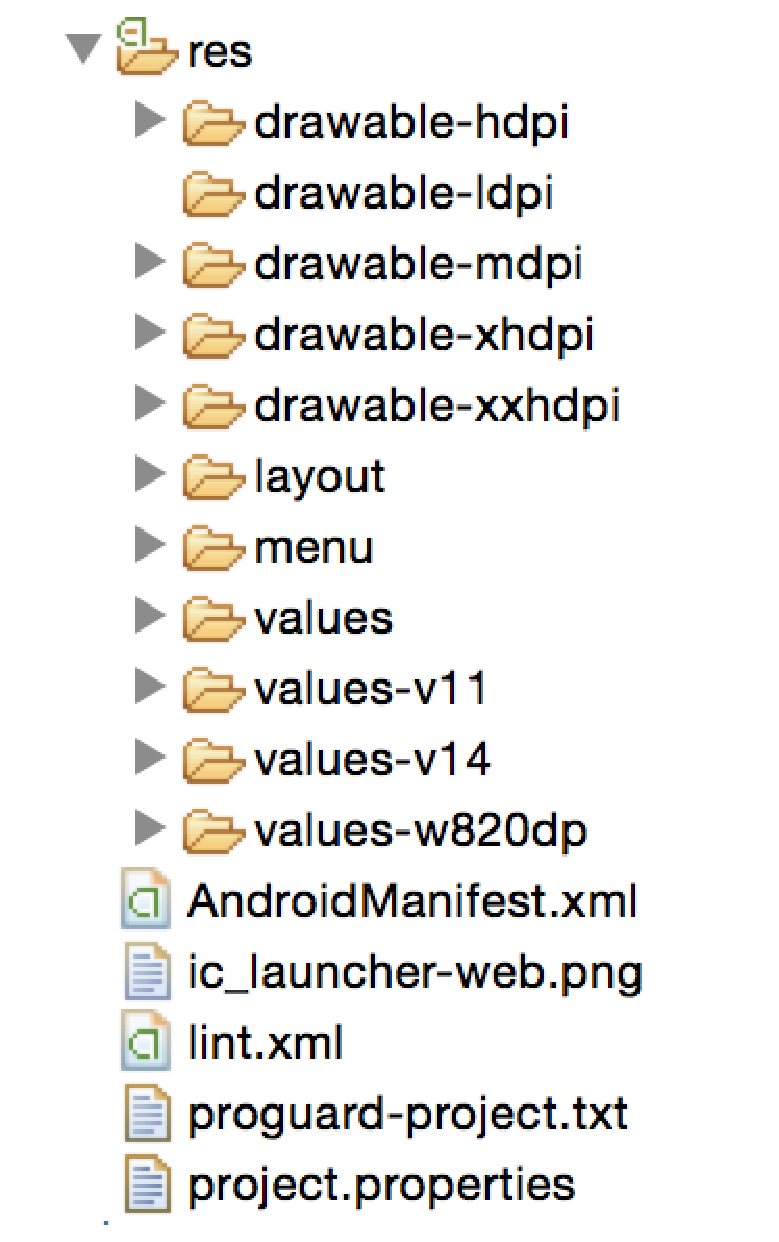
\includegraphics[ scale = 0.2]{resource.eps}
\end{center}
\caption{ res ディレクトリの構成}
\label{res}
\end{figure}

\begin{figure}[t]
\begin{center}
\graphicspath{{./epsfiles/}}
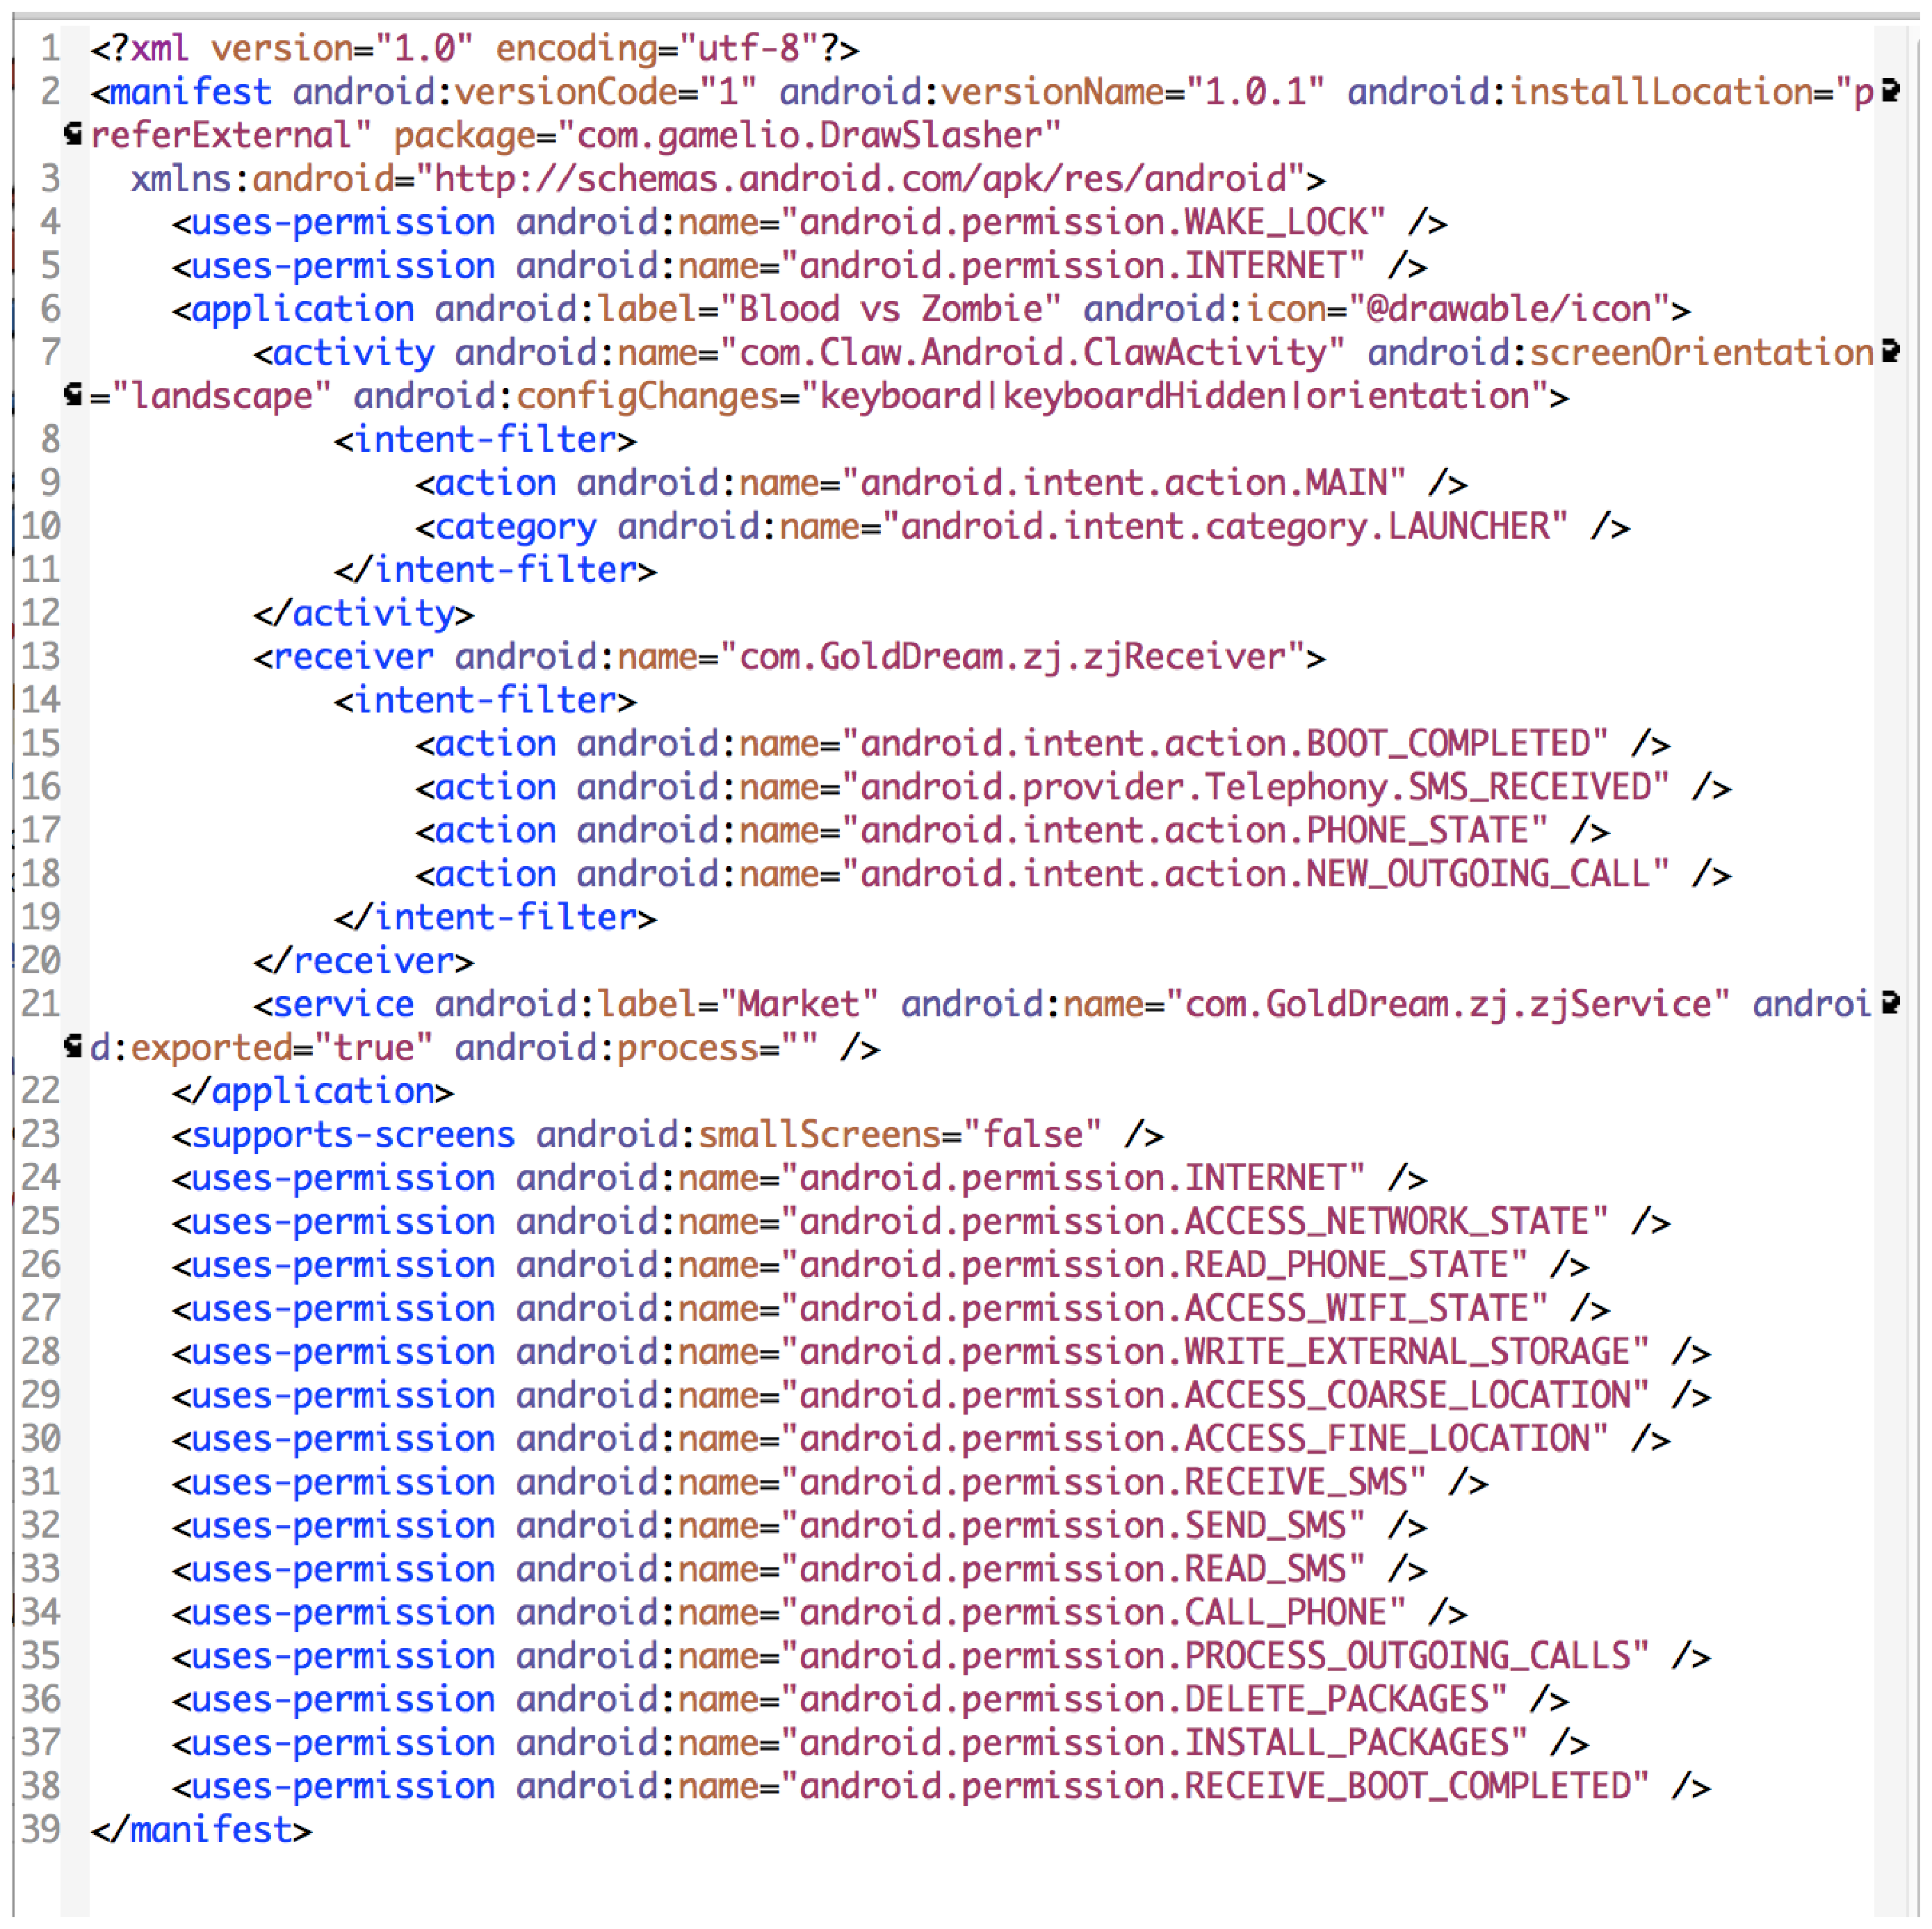
\includegraphics[scale=0.25]{manifest2.eps}
\end{center}
\caption{AndroidManifest.xml の例}
\label{manif}
\end{figure}

